\documentclass[12pt,a4paper]{report}

\usepackage[T1]{fontenc}
\usepackage[utf8]{inputenc}
\usepackage[portuguese]{babel}
\usepackage[a4paper,margin=2.5cm]{geometry}
\usepackage{graphicx}
\usepackage{float}
\usepackage{hyperref}
\usepackage{titlesec}
\usepackage{setspace}
\usepackage{enumitem}

\setstretch{1.15}
\hypersetup{
  colorlinks=true,
  linkcolor=blue,
  urlcolor=blue,
  pdftitle={Trabalho Prático \#1 - BaseballX},
}

\title{Trabalho Pr\'atico \#1\\NBA}
\author{
  Afonso Ferreira - 113480 \\
  Tomás Brás - 112665 \\
  David Pelicano - 113391
}
\date{Web Sem\^antica -- 2024/2025\\Mestrado em Engenharia Inform\'atica}

\begin{document}

\maketitle
\tableofcontents
\listoffigures
\clearpage

\chapter{Introdu\c{c}\~ao ao Tema}

\section{Arquitetura da Aplica\c{c}\~ao e Tecnologias Utilizadas}

Descreva aqui a arquitetura da aplica\c{c}\~ao, o padr\~ao adotado e as tecnologias principais.

\begin{itemize}[leftmargin=*]
  \item Django
  \item GraphDB
  \item SPARQL / SPARQLWrapper
  \item Bibliotecas frontend e visualiza\c{c}\~ao
  \item Docker
\end{itemize}

\chapter{Dados, suas fontes e sua transforma\c{c}\~ao}

A base de conhecimento do projeto parte de um conjunto de ficheiros CSV com informa\c{c}\~ao hist\'orica sobre baseball, armazenados na pasta \texttt{archive/}. Estes dados cobrem entidades centrais, como jogadores, equipas e franquias, mas tamb\'em estat\'isticas sazonais, sal\'arios, pr\'emios e eventos especiais. A sua transforma\c{c}\~ao para RDF permitiu passar de um conjunto de tabelas independentes para um grafo interligado, mais adequado para explora\c{c}\~ao sem\^antica.

\section{Fontes de Dados Principais}

O n\'ucleo do projeto assenta num arquivo hist\'orico de baseball em formato CSV, compat\'ivel com a estrutura cl\'assica da base de dados Lahman. No trabalho foram efetivamente utilizados os seguintes grupos de ficheiros:

\begin{itemize}[leftmargin=*]
  \item \texttt{Master.csv}: identifica\c{c}\~ao dos jogadores e informa\c{c}\~ao biogr\'afica, como nome, data de nascimento, pa\'is de origem, altura, peso, datas de estreia e \'{u}ltimo jogo.
  \item \texttt{Teams.csv}, \texttt{TeamsFranchises.csv} e \texttt{TeamsHalf.csv}: informa\c{c}\~ao sobre equipas, franquias, ligas e desempenho por \'{e}poca ou meia-\'{e}poca.
  \item \texttt{Batting.csv}, \texttt{BattingPost.csv}, \texttt{Pitching.csv}, \texttt{PitchingPost.csv}, \texttt{Fielding.csv} e \texttt{FieldingOF.csv}: estat\'isticas detalhadas de batting, pitching e fielding, tanto na fase regular como na p\'os-temporada.
  \item \texttt{Salaries.csv}: valores salariais por jogador, equipa e ano.
  \item \texttt{AwardsPlayers.csv} e \texttt{AwardsSharePlayers.csv}: pr\'emios individuais e vota\c{c}\~oes associadas aos jogadores.
  \item \texttt{AwardsManagers.csv} e \texttt{AwardsShareManagers.csv}: pr\'emios e vota\c{c}\~oes associados aos managers.
  \item \texttt{HallOfFame.csv} e \texttt{AllstarFull.csv}: vota\c{c}\~oes para o Hall of Fame e participa\c{c}\~oes em All-Star Games.
  \item \texttt{Managers.csv}, \texttt{ManagersHalf.csv} e \texttt{SeriesPost.csv}: hist\'orico de managers e resultados de s\'eries de p\'os-temporada.
\end{itemize}

Este conjunto de fontes foi suficiente para modelar um dom\'inio rico, com rela\c{c}\~oes entre pessoas, equipas, desempenhos desportivos, distin\c{c}\~oes individuais e contexto competitivo ao longo do tempo.

\begin{figure}[H]
  \centering
  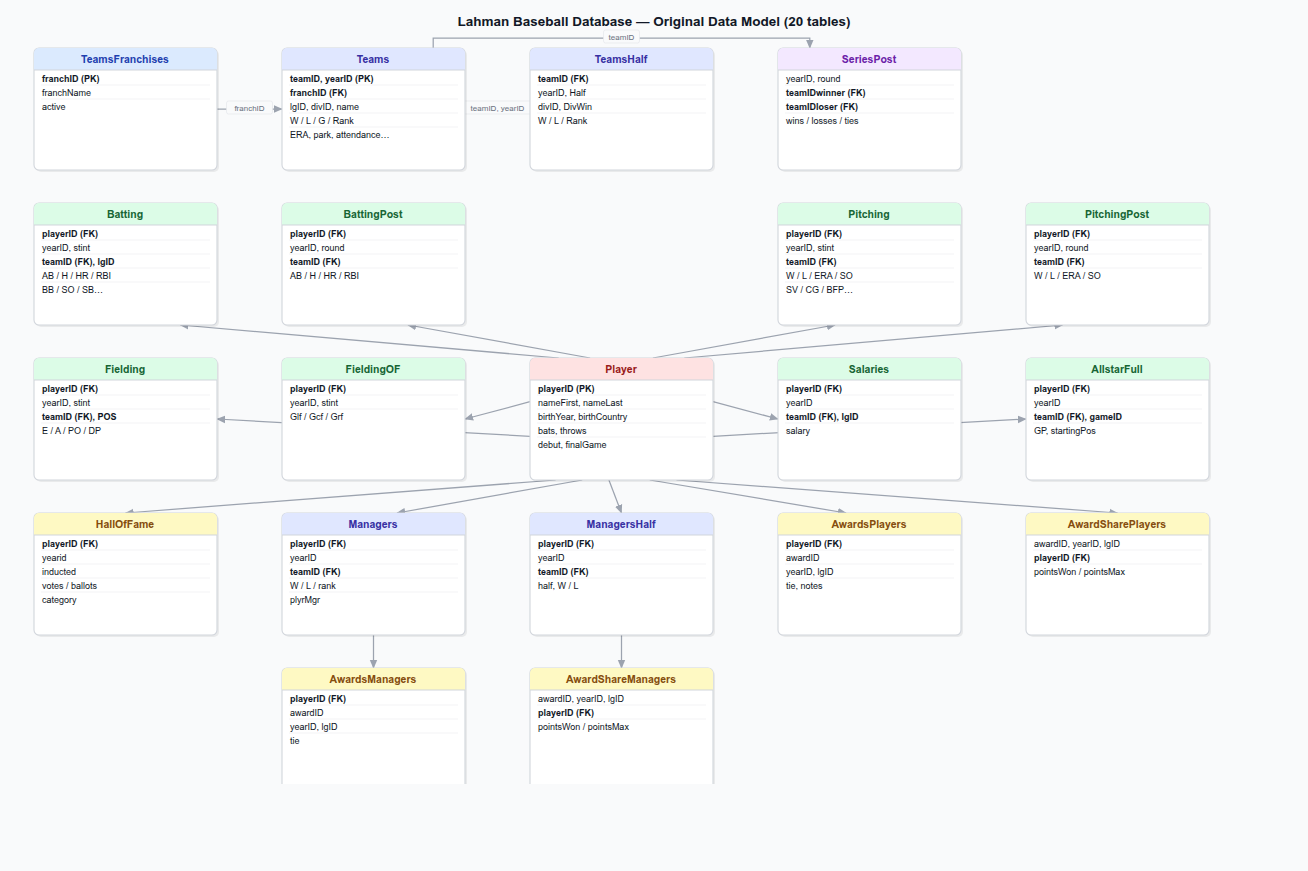
\includegraphics[width=\textwidth]{images/data_model.png}
  \caption{Modelo de dados original baseado nos ficheiros CSV utilizados no projeto.}
  \label{fig:csv_data_model}
\end{figure}

\section{Transforma\c{c}\~ao para RDF}

O processo de transforma\c{c}\~ao foi implementado no script \texttt{rdf/convert.py}. Esse script percorre cada CSV com \texttt{csv.DictReader}, extrai os atributos relevantes e cria recursos RDF com base no namespace \texttt{http://baseball.ws.pt/}. Para cada tipo de entidade \'{e} gerada uma URI est\'avel e leg\'ivel, sendo aplicadas regras de normaliza\c{c}\~ao para evitar caracteres problem\'aticos nos identificadores.

Durante a convers\~ao s\~ao declaradas classes para jogadores, franquias, equipas, estat\'isticas desportivas, sal\'arios, pr\'emios, Hall of Fame, All-Star Games e managers. Em seguida, cada linha dos CSV origina inst\^ancias dessas classes e \'{e} ligada \`as restantes entidades atrav\'es de propriedades sem\^anticas. Por exemplo, um jogador pode ficar associado a batting, pitching, fielding, sal\'arios, pr\'emios e apari\c{c}\~oes em All-Star Games, enquanto cada estat\'istica fica ligada \`a equipa e ao ano respetivos.

\begin{itemize}[leftmargin=*]
  \item Os valores num\'ericos s\~ao convertidos para literais tipados, principalmente \texttt{xsd:integer} e \texttt{xsd:decimal}.
  \item Datas relevantes, como estreia e \'{u}ltimo jogo, s\~ao representadas com \texttt{xsd:date}.
  \item Campos l\'ogicos, como vit\'oria de divis\~ao ou entrada no Hall of Fame, s\~ao convertidos para \texttt{xsd:boolean}.
  \item Valores vazios, inconsistentes ou marcados como \texttt{NA}, \texttt{null} e equivalentes s\~ao ignorados para evitar ru\'ido no grafo.
  \item O nome leg\'ivel do jogador \'{e} adicionalmente exposto com \texttt{foaf:name}, facilitando as consultas e a apresenta\c{c}\~ao na interface.
\end{itemize}

O resultado final desta transforma\c{c}\~ao \'{e} o ficheiro \texttt{rdf/baseball.n3}, em formato N3. Esse ficheiro \'{e} depois importado para um reposit\'orio \texttt{baseball} no GraphDB, onde passa a estar dispon\'ivel para consulta atrav\'es de SPARQL pela aplica\c{c}\~ao Django.

\begin{figure}[H]
  \centering
  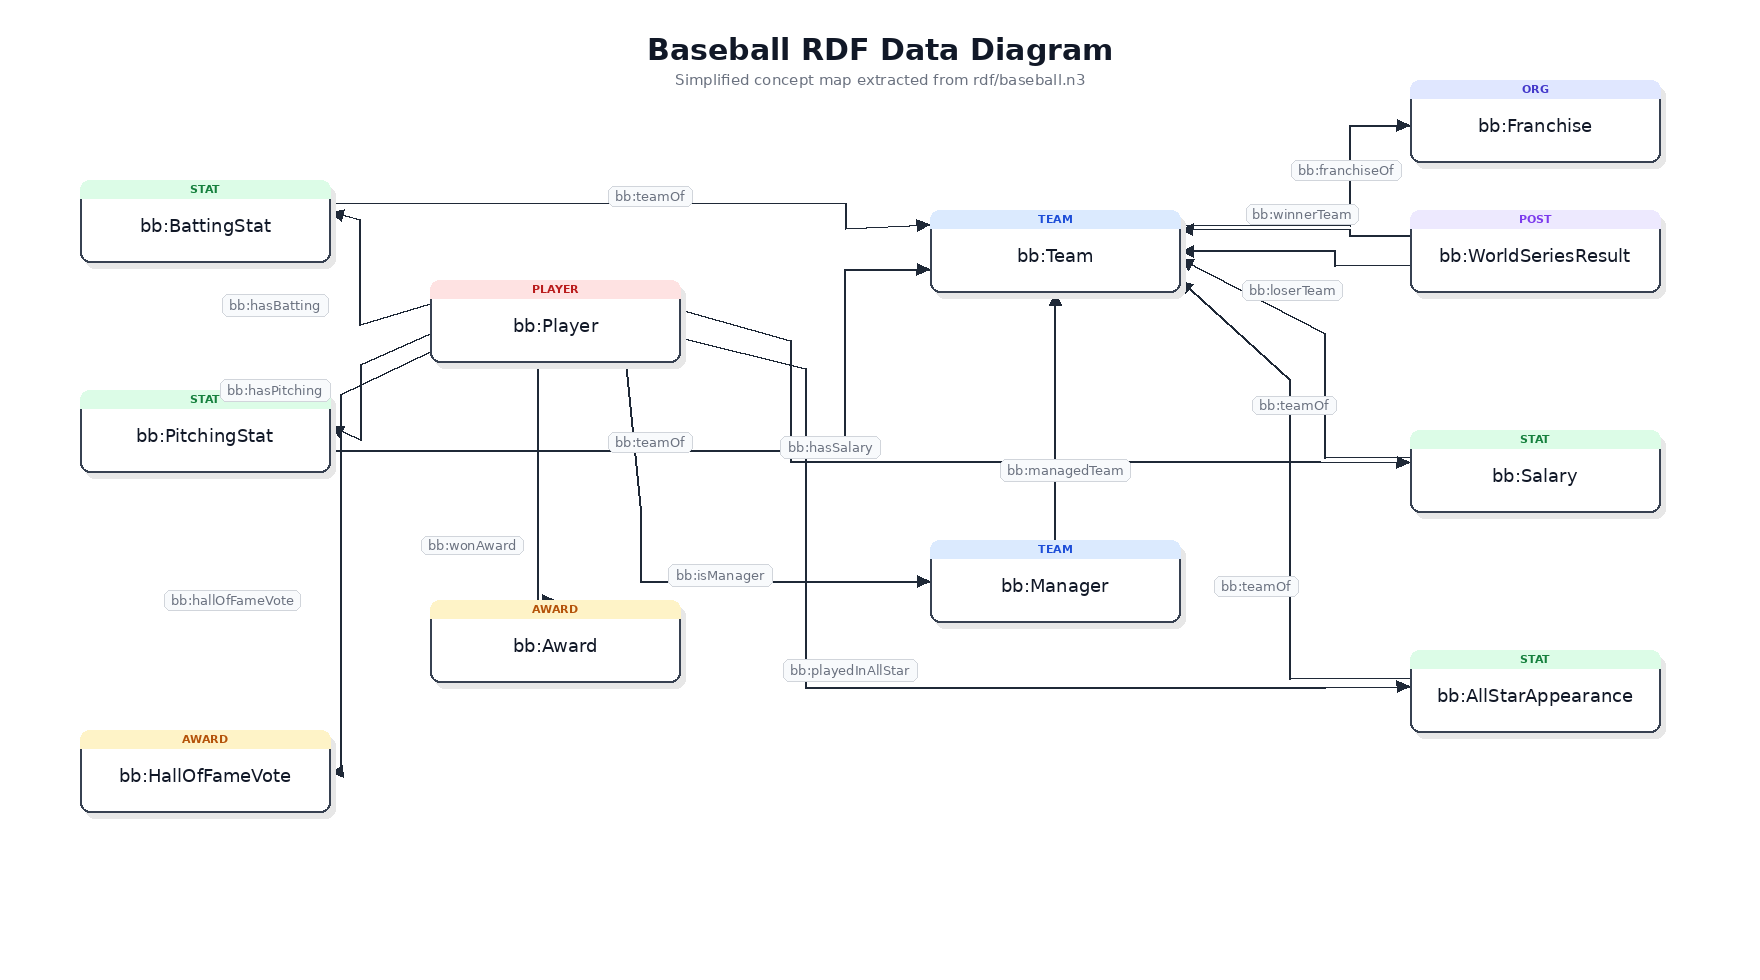
\includegraphics[width=\textwidth]{images/rdf_data_model.png}
  \caption{Vis\~ao simplificada do modelo RDF resultante, destacando as principais classes e rela\c{c}\~oes materializadas no grafo.}
  \label{fig:rdf_data_model}
\end{figure}

\section{Decis\~oes de Modela\c{c}\~ao, Limpeza e Exclus\~ao}

Embora os dados de origem sejam ricos, o arquivo original encontra-se organizado como um conjunto de tabelas CSV independentes, com conven\c{c}\~oes herdadas da base de dados Lahman e com alguns problemas t\'ipicos de dados hist\'oricos: valores omissos, variantes de c\'odigos, flags representadas por letras, colunas redundantes e diferentes n\'iveis de detalhe conforme o ficheiro. Por isso, antes da gera\c{c}\~ao do grafo RDF, foi necess\'ario tomar algumas decis\~oes expl\'icitas de normaliza\c{c}\~ao e de desenho do modelo.

\subsection{Como os dados originais foram interpretados}

Cada ficheiro CSV foi tratado como uma fonte de uma entidade ou rela\c{c}\~ao principal do dom\'inio:

\begin{itemize}[leftmargin=*]
  \item \texttt{Master.csv} foi usado como fonte can\'onica para jogadores, porque concentra o identificador principal (\texttt{playerID}) e os atributos biogr\'aficos mais est\'aveis.
  \item \texttt{Teams.csv} e \texttt{TeamsFranchises.csv} foram usados para distinguir duas no\c{c}\~oes diferentes: a equipa numa dada \'{e}poca e a franquia enquanto entidade hist\'orica.
  \item Os ficheiros de batting, pitching, fielding, sal\'arios, pr\'emios, Hall of Fame, All-Star e managers foram interpretados como ocorr\^encias temporais ligadas a um jogador e, quando aplic\'avel, a uma equipa e a um ano.
  \item Nos casos em que o significado do registo dependia de mais do que um identificador, a URI RDF passou a incorporar essas componentes. Por exemplo, as estat\'isticas usam combina\c{c}\~oes como jogador + ano + stint, e as equipas usam equipa + ano.
\end{itemize}

Esta decis\~ao evita colis\~oes entre recursos e preserva o car\'acter temporal do dataset original, que \'{e} central para o dom\'inio desportivo.

\subsection{Regras de limpeza e normaliza\c{c}\~ao}

O script \texttt{rdf/convert.py} n\~ao se limita a copiar os valores dos CSV para RDF. Antes disso, aplica um conjunto pequeno, mas importante, de regras de limpeza:

\begin{itemize}[leftmargin=*]
  \item Espa\c{c}os em branco repetidos s\~ao removidos e o texto \'{e} aparado para evitar diferen\c{c}as artificiais entre valores semanticamente iguais.
  \item C\'odigos como \texttt{teamID}, \texttt{lgID}, \texttt{franchID} e \texttt{divID} s\~ao normalizados para mai\'usculas, tornando as refer\^encias mais consistentes.
  \item Alguns pa\'ises aparecem com variantes no arquivo original, como \texttt{USA}, \texttt{US} ou \texttt{U.S.A.}; essas variantes foram consolidadas numa forma comum, como \texttt{United States}.
  \item Flags como \texttt{Y}/\texttt{N}, \texttt{TRUE}/\texttt{FALSE} e variantes equivalentes s\~ao convertidas para booleanos RDF.
  \item Valores vazios ou marcadores como \texttt{NA}, \texttt{N/A}, \texttt{null}, \texttt{none} e semelhantes n\~ao s\~ao materializados no grafo.
  \item Datas, inteiros e decimais s\~ao tipados explicitamente com \texttt{xsd:date}, \texttt{xsd:integer} e \texttt{xsd:decimal}, o que simplifica consultas e ordena\c{c}\~oes em SPARQL.
  \item Os componentes usados nas URIs passam por uma sanitiza\c{c}\~ao simples, removendo caracteres problem\'aticos e garantindo identificadores est\'aveis.
\end{itemize}

Na pr\'atica, esta fase reduz ru\'ido no grafo e evita que diferen\c{c}as de formata\c{c}\~ao nos CSV comprometam a liga\c{c}\~ao entre entidades.

\subsection{Decis\~oes de modela\c{c}\~ao RDF}

Também fora tomadas algumas decis\~oes para tornar o grafo mais f\'acil de consultar a partir da aplica\c{c}\~ao:

\begin{itemize}[leftmargin=*]
  \item Foram introduzidas propriedades mais leg\'iveis e diretamente \'{u}teis para a interface, como \texttt{bb:teamName}, \texttt{bb:franchiseName} e \texttt{bb:awardName}, mesmo quando essas informa\c{c}\~oes j\'a existiam noutras colunas equivalentes.
  \item Tamb\'em foram expostos atalhos sem\^anticos para estat\'isticas frequentes, como \texttt{bb:homeRuns}, \texttt{bb:wins}, \texttt{bb:losses} e \texttt{bb:rank}, de modo a simplificar consultas e a camada de apresenta\c{c}\~ao.
  \item O nome do jogador foi exposto tamb\'em com \texttt{foaf:name}, o que facilita a apresenta\c{c}\~ao textual e aproxima o modelo de vocabul\'arios mais comuns da Web Sem\^antica.
  \item As rela\c{c}\~oes entre recursos foram materializadas explicitamente com propriedades como \texttt{bb:hasBatting}, \texttt{bb:hasPitching} e \texttt{bb:hasSalary}.
  \item O mesmo princ\'ipio foi usado para liga\c{c}\~oes de contexto, como \texttt{bb:wonAward}, \texttt{bb:managedTeam} e \texttt{bb:franchiseOf}. Isto torna as consultas mais diretas do que depender apenas de chaves literais repetidas.
\end{itemize}

Estas decis\~oes privilegiam legibilidade e simplicidade de consulta em vez de um minimalismo ontol\'ogico estrito.

\subsection{Dados exclu\'idos por omiss\~ao e justifica\c{c}\~ao}

O conversor suporta dois perfis: \texttt{lean} e \texttt{full}. O perfil \texttt{full} exporta todas as vinte tabelas modeladas no projeto, enquanto o perfil \texttt{lean} \textemdash{} usado por omiss\~ao \textemdash{} exporta apenas o subconjunto atualmente necess\'ario para a aplica\c{c}\~ao Web e para as consultas principais.

No perfil \texttt{lean}, ficam fora do RDF final importado por omiss\~ao os seguintes conjuntos:

\begin{itemize}[leftmargin=*]
  \item \texttt{TeamsHalf.csv}
  \item \texttt{BattingPost.csv} e \texttt{PitchingPost.csv}
  \item \texttt{AwardsSharePlayers.csv}
  \item \texttt{Fielding.csv} e \texttt{FieldingOF.csv}
  \item \texttt{ManagersHalf.csv}
  \item \texttt{AwardsManagers.csv} e \texttt{AwardsShareManagers.csv}
\end{itemize}

Ested dados não eram s\~ao necess\'arios para as funcionalidades da interface atual e, por isso, a sua omiss\~ao reduz o tamanho do grafo, acelera a importa\c{c}\~ao no GraphDB e torna as consultas mais rápidas. 


\section{Dados Complementares para a Interface}

Para al\'em do grafo RDF principal, o projeto inclui uma pequena camada de enriquecimento visual para a interface. A partir do identificador \texttt{bbrefID} presente em \texttt{Master.csv}, foram usados scripts auxiliares para construir cat\'alogos JSON com fotografias de jogadores, recorrendo a URLs do Baseball-Reference e a imagens disponibilizadas pela MLB. Da mesma forma, os log\'otipos atuais das equipas s\~ao resolvidos atrav\'es de identificadores est\'aticos da MLB.

Estes dados complementares n\~ao fazem parte do n\'ucleo sem\^antico armazenado no GraphDB, mas melhoram a experi\^encia de utiliza\c{c}\~ao da aplica\c{c}\~ao, sobretudo nas p\'aginas de detalhe, listagens de jogadores e visualiza\c{c}\~oes gr\'aficas.

\chapter{Opera\c{c}\~oes sobre os dados (SPARQL)}

Documente aqui as queries SPARQL principais, objetivo de cada query e resultados obtidos.

\section*{Exemplo de Estrutura}
\begin{itemize}[leftmargin=*]
  \item Query 1: objetivo, consulta e interpreta\c{c}\~ao do resultado.
  \item Query 2: objetivo, consulta e interpreta\c{c}\~ao do resultado.
  \item Query N: objetivo, consulta e interpreta\c{c}\~ao do resultado.
\end{itemize}

\chapter{Funcionalidades da Aplica\c{c}\~ao (UI)}

Descreva as funcionalidades de interface e a navega\c{c}\~ao do utilizador.

\section*{Sugest\~ao}
Insira as capturas de ecr\~a numeradas para reproduzir a lista de figuras (4.1 a 4.24).

\chapter{Funcionalidades de Administrador (Autentica\c{c}\~ao e Opera\c{c}\~oes CRUD)}


\chapter{Conclus\~oes}

Resuma os resultados, desafios encontrados e melhorias futuras.

\chapter{Configura\c{c}\~oes para executar a app}

\section{Vis\~ao geral}

Para executar o projeto BaseBallX s\~ao necess\'arios tr\^es elementos principais:

\begin{itemize}[leftmargin=*]
  \item um ambiente Python com as depend\^encias da aplica\c{c}\~ao;
  \item um reposit\'orio \texttt{baseball} ativo no GraphDB;
  \item a aplica\c{c}\~ao Django a correr localmente.
\end{itemize}

O fluxo de execu\c{c}\~ao pode ser resumido da seguinte forma:

\begin{enumerate}[leftmargin=*]
  \item criar e ativar o ambiente virtual Python;
  \item instalar depend\^encias;
  \item gerar o ficheiro RDF \texttt{rdf/baseball.n3};
  \item iniciar o GraphDB e carregar o reposit\'orio \texttt{baseball};
  \item aplicar as migrations do Django;
  \item iniciar o servidor web.
\end{enumerate}

\section{Pr\'e-requisitos}

Antes da execu\c{c}\~ao, o sistema deve ter instalado:

\begin{itemize}[leftmargin=*]
  \item \textbf{Python 3};
  \item \textbf{GraphDB Desktop}
  \item \textbf{curl}, usado pelos scripts auxiliares;
  \item acesso ao diret\'orio do projeto com os dados na pasta \texttt{archive/}.
\end{itemize}

Garantir que a porta \texttt{7200} est\'a livre para o GraphDB 
\begin{center}
\texttt{http://localhost:7200}
\end{center}

\section{Execu\c{c}\~ao manual}

\subsection{1. Criar o ambiente virtual}

Na raiz do projeto:

\begin{verbatim}
python3 -m venv venv
source venv/bin/activate
pip install -r requirements.txt
\end{verbatim}

\subsection{2. Gerar o RDF}

Se o ficheiro RDF ainda n\~ao existir deve ser executada a convers\~ao:

\begin{verbatim}
python3 rdf/convert.py
\end{verbatim}

Este comando gera o ficheiro:

\begin{center}
\texttt{rdf/baseball.n3}
\end{center}

\subsection{3. Iniciar o GraphDB e criar o reposit\'orio}

Existem duas formas de preparar o GraphDB.

\textbf{Op\c{c}\~ao A: usar o script auxiliar}

\begin{verbatim}
./scripts/start_graphdb.sh
\end{verbatim}

Este script:

\begin{itemize}[leftmargin=*]
  \item verifica se o GraphDB est\'a acess\'ivel;
  \item tenta abrir o GraphDB Desktop se o servi\c{c}o ainda n\~ao estiver ativo;
  \item cria o reposit\'orio \texttt{baseball} se este ainda n\~ao existir;
  \item importa automaticamente o ficheiro \texttt{rdf/baseball.n3}.
\end{itemize}

Por omiss\~ao, o script usa:

\begin{itemize}[leftmargin=*]
  \item \texttt{GRAPHDB\_URL=http://localhost:7200}
  \item \texttt{REPOSITORY\_ID=baseball}
  \item \texttt{RDF\_FILE=\$ROOT\_DIR/rdf/baseball.n3}
  \item \texttt{GRAPHDB\_DESKTOP\_BIN=/opt/graphdb-desktop/bin/graphdb-desktop}
\end{itemize}

% \textbf{Op\c{c}\~ao B: fazer manualmente no GraphDB Desktop}
% 
% \begin{enumerate}[leftmargin=*]
%   \item abrir o GraphDB Desktop;
%   \item iniciar o servi\c{c}o local;
%   \item criar um reposit\'orio com o nome \texttt{baseball};
%   \item importar o ficheiro \texttt{rdf/baseball.n3} para esse reposit\'orio.
% \end{enumerate}
% 
% \subsection{4. Preparar a base de dados Django}

A aplica\c{c}\~ao usa SQLite para persistir contas, sugest\~oes, sess\~oes e resultados do quiz. Depois de ativar o ambiente virtual, devem ser aplicadas as migrations:

\begin{verbatim}
cd webapp
python manage.py migrate
\end{verbatim}

\subsection{5. Iniciar o servidor web}

Ainda na pasta \texttt{webapp}, iniciar a aplica\c{c}\~ao Django:

\begin{verbatim}
python manage.py runserver
\end{verbatim}

Depois disso, a aplica\c{c}\~ao fica dispon\'ivel em:

\begin{center}
\texttt{http://127.0.0.1:8000/}
\end{center}

\section{Fluxo completo recomendado}

O fluxo mais direto para executar o projeto desde o in\'icio \'{e}:

\begin{verbatim}
python3 -m venv venv
source venv/bin/activate
pip install -r requirements.txt
python3 rdf/convert.py
./scripts/start_graphdb.sh
cd webapp
python manage.py migrate
python manage.py runserver
\end{verbatim}

\section{Parar e reconstruir o reposit\'orio}

Se for necess\'ario apagar o reposit\'orio do GraphDB e voltar a import\'a-lo, existe um script dedicado:

\begin{verbatim}
./scripts/delete_graphdb_repo.sh
\end{verbatim}

Depois da remo\c{c}\~ao, basta correr novamente:

\begin{verbatim}
./scripts/start_graphdb.sh
\end{verbatim}

Isto volta a criar o reposit\'orio \texttt{baseball} e a importar o ficheiro RDF.


\end{document}
